% Chapter Template

\chapter{OpenCL} % Main chapter title

\label{Chapter4} % Change X to a consecutive number; for referencing this chapter elsewhere, use \ref{ChapterX}

%----------------------------------------------------------------------------------------
%	SECTION 1
%----------------------------------------------------------------------------------------

\section{History and Introduction}

With the predictions of the Moore's Law \cite{moore1965cramming} coming to an end for single-core processors, new programming and hardware paradigm was needed to continue the exponential growth. Increasing the frequency of the chip to improve performance would have resulted in overheating (Power Wall). Furthermore, manufacturers continued to reduce the size of a transistor, giving them more computing elements to work with. The answer was reducing the frequency, but using extra transistors to exploit various levels of parallelism present in programs.\\
\\
CPU manufactures (Intel, AMD) needed to maintain the performance of single-threaded applications intact, while expoliting thread-level parallelism. They opted to have a small number of independent cores in their processors (eg. Intel Dual Core). This was complemented by the invention of hyperthreading \cite{marr2002hyper}, which enabled a single core to execute multiple instruction streams simultaneously, reducing the number of unused circuits.\\
\\
GPU computing took a different route \cite{mcclanahan2010history}. GPU loads were already massively parallel - small programs were applied to every pixel on the screen. This resulted in GPUs having hundreds of small processor, performing the same computation on different data (SIMD - Single Instruction Multiple Data). Unfortunately, even though their computing power continued to grow, graphics cards were limited to performing only computations limited to image processing. This changed with OpenGL 2.0 standard released in 2004 \cite{segal2004opengl}. Even though OpenGL is a graphics API, it enabled users to write general-purpose code using GLSL \cite{kessenich2004opengl}. Soon, NVIDIA published their own general-purpose GPU solution - CUDA \cite{nvidia2007nvidia}.\\
\\
With so much different parallel hardware on the market, interoperability was hard to achieve. Someone having an ATI GPU could not run CUDA programs, so they were forced to buy a new graphics card, or port their software to OpenGL 2.0 which was meant to be used for graphics. In 2009. Apple published OpenCL to provide heterogenous computing support on as many platforms as possible. Only OpenCL architecture is standardized, so the actual, underlying implementation (organization) is left to hardware vendors. This means that OpenCL programs can take full advantage of available hardware - GPUs will execute them in SIMD fashion, FPGA compilers will create only needed SIMD hardware, while multi-core CPUs will run the program in multiple threads. Today, OpenCL is supported on multi-core CPUs, integrated CPU graphics, GPUs, FPGAs, and by almost all major hardware manufacturers (Intel, AMD, NVIDIA, ARM...).


%----------------------------------------------------------------------------------------
%	SECTION 2
%----------------------------------------------------------------------------------------

\section{OpenCL Architecture}

Information in this section is based on \cite{gaster2012heterogeneous}.

\subsection{Host and Kernel}

OpenCL program consists of two parts: host program and a guest program (kernel) (Figure \ref{fig:openclplatform}). Host program is written in a language which has OpenCL bindings available (C, C++, Python, Rust\dots), while the kernel is written in OpenCL C or OpenCL C++ (OpenCL 2.1+). Host application interfaces with the operating system to find out which OpenCL devices are available, compiles kernels, queues them for execution and reads back the result. Kernel receives parameters from the host application, performs (usually parallel) operations and returns the result.

\begin{figure}[h]
    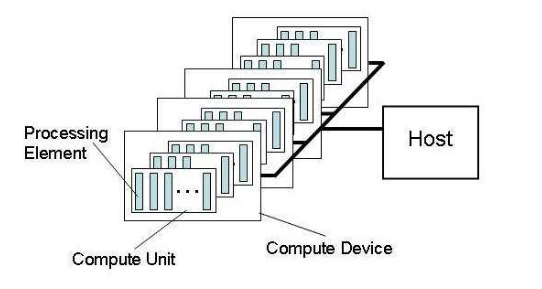
\includegraphics[width=\linewidth]{Figures/platform.png}
    \caption{OpenCL Platform Model\cite{munshi2009opencl}}
    \label{fig:openclplatform}
\end{figure}

To help parallelization, many instances of kernel are run, each having a different ID. Based on its ID, kernel decided which data to fetch, and which operations to execute. Several kernel instances can form a group, which can be used to partially synchronize execution of more complex kernel. Host program determines the total number of kernel instances, as well as the size of a group.

\subsection{Memory Hierarchy}
OpenCL was heavily influenced by CUDA, which is evident in the organization of memory (Figure \ref{fig:openclmemory}). While CPUs usually automatically handle latency hiding by caching frequent accesses, there are no guarantees that OpenCL devices have cache on-board. The developer must choose where data resides.

\begin{figure}[h]
    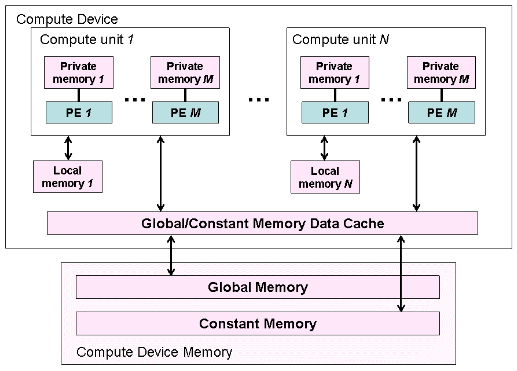
\includegraphics[width=\linewidth]{Figures/memory.png}
    \caption{OpenCL Memory Model\cite{munshi2009opencl}}
    \label{fig:openclmemory}
\end{figure}

There are three levels of memory, each smaller, faster and accessible by a smaller number of elements than the last. Devices differ in the amount of memory available at each level. If kernel uses more memory than available, accesses will spill to a lower memory level, slowing down memory accesses.
\begin{itemize}
    \item \b{Global memory} (\texttt{\_\_global}) is accessible by every kernel instance, as well as by a host application (using OpenCL calls). This is where host usually writes starting data, and where kernel outputs results. It has the longest latency, but also the highest capacity. \b{Constant memory} (\texttt{\_\_constant}) is a special part of global memory where read-only data can be stored.
    \item \b{Local memory} (\texttt{\_\_local}) is accessible by the elements in the same group.
    \item \b{Private memory} (no keyword) is accessible only by its owner. It is the fastest, but also the smallest memory.
\end{itemize}

\subsection{Latency Hiding}

While OpenCL is indeed platform-agnostic, organizational details of GPUs affect performance of OpenCL code running on them. GPUs consist of thousands of compute units split in groups which execute same instructions in parallel. When a unit issues a data request, the thread blocks until it is served. If there is free space in the register file, the scheduler will start the execution of the next segment. This can happen as many times as needed, as long as there are free registers. If a kernel is well optimized, the GPU will almost never be idle.\\
\\
This leads to two opposite concepts to keep in mind when writing OpenCL kernels for GPUs. Caching frequently used data in local and private memory (without overflowing to lower hierarchies) reduces latency for subsequent accesses. Unfortunately, this also reduces the number of threads whose state we can keep simultaneously. Balancing these two forces leads to fastest execution of a kernel.\\
% The following sentence should be moved to the chapter about implementation
%Today, OpenCL compilers often use LLVM and perform many different optimization runs on kernel code. Hand-optimizing register usage to an extent that makes code unreadable, as well as performing trivial changes in the code, should be avoided because compilers will usually generate the same code. Developers should focus on things compilers can't and shouldn't optimize - algorithmic improvements and use of memory hierarchy.
